% arXiv preprint. Build: `make paper` (figures, then LaTeX). arXiv compiles with pdfLaTeX, so the
% preamble uses pdfLaTeX packages only. Numbers come from generated/numbers.tex, never typed by hand.
\documentclass[10pt]{article}

% ---- Page and type -------------------------------------------------------------------------------
\usepackage[letterpaper, margin=1in]{geometry}
\usepackage{iftex, amsmath}
\ifPDFTeX                                     % arXiv (pdfLaTeX): Type 1 fonts
  \usepackage[T1]{fontenc}
  \usepackage{libertinus}                     % text + maths; sans for headings
  \usepackage[scaled=0.9]{zi4}                % Inconsolata mono, sized to the text
  \usepackage{amssymb}
\else                                         % local build (tectonic = XeTeX): the same fonts as OpenType
  \usepackage{libertinus}                     % loads unicode-math, which already has amssymb's symbols
\fi
\usepackage[final]{microtype}
\linespread{1.06}
\setlength{\parskip}{0.35em}
\setlength{\parindent}{0pt}

% ---- Colour, links, references -------------------------------------------------------------------
\usepackage{xcolor}
\definecolor{encoder}{HTML}{2A78D6}           % = figures/style.py ENCODER
\definecolor{decoder}{HTML}{EB6834}           % = figures/style.py DECODER
\definecolor{ink2}{HTML}{52514E}
\usepackage[colorlinks, linkcolor=encoder, citecolor=encoder, urlcolor=encoder]{hyperref}
\usepackage[capitalise, noabbrev]{cleveref}
\usepackage[numbers, sort&compress]{natbib}

% ---- Headings and captions: sans, quiet ---------------------------------------------------------
\usepackage[sf, bf, small, compact]{titlesec}
\titlespacing*{\section}{0pt}{1.4em}{0.5em}
\titlespacing*{\subsection}{0pt}{1em}{0.3em}
\usepackage[font=small, labelfont={sf, bf}, labelsep=period, skip=5pt]{caption}

% ---- Tables, figures, maths ----------------------------------------------------------------------
\usepackage{booktabs, graphicx}
\usepackage{tikz}
\usetikzlibrary{positioning, arrows.meta, fit, calc}
\graphicspath{{generated/}}
% Generated by paper/figures/make_figures.py; do not edit.
\newcommand{\TestUbSig}{72.1}
\newcommand{\TestUbSigCI}{[71.0, 73.0]}
\newcommand{\DevUbSig}{72.7}
\newcommand{\ExtUbSig}{59.5}
\newcommand{\TestUbList}{69.7}
\newcommand{\TestUbListCI}{[68.7, 70.7]}
\newcommand{\DevUbList}{71.2}
\newcommand{\ExtUbList}{57.8}
\newcommand{\TestQwFull}{67.6}
\newcommand{\TestQwFullCI}{[66.5, 68.7]}
\newcommand{\DevQwFull}{69.0}
\newcommand{\ExtQwFull}{56.1}
\newcommand{\TestQwLora}{63.0}
\newcommand{\TestQwLoraCI}{[61.7, 64.3]}
\newcommand{\DevQwLora}{64.5}
\newcommand{\ExtQwLora}{56.9}
\newcommand{\TestQwFourLora}{77.3}
\newcommand{\TestQwFourLoraCI}{[76.2, 78.4]}
\newcommand{\DevQwFourLora}{79.3}
\newcommand{\ExtQwFourLora}{73.5}
\newcommand{\DiffUbSigQwFull}{+4.4}
\newcommand{\DiffUbSigQwFullCI}{[+3.3, +5.5]}
\newcommand{\DiffUbSigQwFullAbs}{4.4}
\newcommand{\DiffUbListQwFull}{+2.1}
\newcommand{\DiffUbListQwFullCI}{[+1.0, +3.1]}
\newcommand{\DiffUbListQwFullAbs}{2.1}
\newcommand{\DiffUbSigUbList}{+2.3}
\newcommand{\DiffUbSigUbListCI}{[+1.7, +2.9]}
\newcommand{\DiffUbSigUbListAbs}{2.3}
\newcommand{\DiffQwFullQwLora}{+4.6}
\newcommand{\DiffQwFullQwLoraCI}{[+3.6, +5.5]}
\newcommand{\DiffQwFullQwLoraAbs}{4.6}
\newcommand{\DiffUbSigQwLoraText}{9.0}
\newcommand{\EvSentAPList}{0.56}
\newcommand{\EvTokAPList}{0.40}
\newcommand{\EvTopOneList}{56}
\newcommand{\EvPTenList}{0.48}
\newcommand{\EvChanceList}{0.17}
\newcommand{\EvMsList}{67}
\newcommand{\EvThrList}{0.73}
\newcommand{\EvWordPList}{0.24}
\newcommand{\EvWordRList}{0.32}
\newcommand{\EvSentAPGold}{0.52}
\newcommand{\EvTokAPGold}{0.39}
\newcommand{\EvTopOneGold}{48}
\newcommand{\EvPTenGold}{0.45}
\newcommand{\EvChanceGold}{0.17}
\newcommand{\EvMsGold}{71}
\newcommand{\EvSentAPSig}{0.68}
\newcommand{\EvTokAPSig}{0.46}
\newcommand{\EvTopOneSig}{74}
\newcommand{\EvPTenSig}{0.61}
\newcommand{\EvChanceSig}{0.17}
\newcommand{\EvMsSig}{75}
\newcommand{\EvThrSig}{0.78}
\newcommand{\EvWordPSig}{0.33}
\newcommand{\EvWordRSig}{0.35}
\newcommand{\AtTwoSentAP}{0.33}
\newcommand{\AtTwoTopOne}{22}
\newcommand{\AtTwoLds}{0.18}
\newcommand{\AtTwoMs}{47}
\newcommand{\ContextCiteSentAP}{0.41}
\newcommand{\ContextCiteTopOne}{45}
\newcommand{\ContextCiteLds}{0.65}
\newcommand{\ContextCiteMs}{1{,}704}
\newcommand{\MsUb}{29}
\newcommand{\MsQwFull}{94}
\newcommand{\MsQwFourLora}{170}
\newcommand{\RpsUb}{76.9}
\newcommand{\RpsQwFull}{16.4}
\newcommand{\RpsQwFourLora}{6.5}
\newcommand{\NTrain}{13{,}000}
\newcommand{\NHeldOut}{6{,}315}
\newcommand{\NDev}{1{,}300}
\newcommand{\MaxTokens}{10{,}240}
\newcommand{\NPerDataset}{1{,}000}
\newcommand{\NTest}{5{,}015}

% Generated by paper/figures/make_figures.py; do not edit.
\newcommand{\CpAccYes}{71.4}
\newcommand{\CpShufYes}{15.6}
\newcommand{\CpDropYes}{5.9}
\newcommand{\CpGradYes}{842}
\newcommand{\CpLabelYes}{0.167}
\newcommand{\CpPosYes}{0.050}
\newcommand{\CpEceYes}{0.038}
\newcommand{\CpAbsSYes}{60.5}
\newcommand{\CpSigGoldYes}{0.000}
\newcommand{\CpSigWrongYes}{0.000}
\newcommand{\CpLabelMusiqueYes}{0.09}
\newcommand{\CpLabelCnliYes}{0.12}
\newcommand{\CpSeedsYes}{3}
\newcommand{\CpAccYesNo}{71.5}
\newcommand{\CpShufYesNo}{12.7}
\newcommand{\CpDropYesNo}{4.3}
\newcommand{\CpGradYesNo}{226}
\newcommand{\CpLabelYesNo}{0.219}
\newcommand{\CpPosYesNo}{0.048}
\newcommand{\CpEceYesNo}{0.030}
\newcommand{\CpAbsSYesNo}{3.1}
\newcommand{\CpSigGoldYesNo}{0.920}
\newcommand{\CpSigWrongYesNo}{0.104}
\newcommand{\CpLabelMusiqueYesNo}{0.17}
\newcommand{\CpLabelCnliYesNo}{0.15}
\newcommand{\CpSeedsYesNo}{1}
\newcommand{\CpAccSig}{72.9}
\newcommand{\CpShufSig}{13.7}
\newcommand{\CpDropSig}{4.9}
\newcommand{\CpGradSig}{190}
\newcommand{\CpLabelSig}{0.139}
\newcommand{\CpPosSig}{0.041}
\newcommand{\CpEceSig}{0.023}
\newcommand{\CpAbsSSig}{7.4}
\newcommand{\CpSigGoldSig}{0.049}
\newcommand{\CpSigWrongSig}{0.001}
\newcommand{\CpLabelMusiqueSig}{0.07}
\newcommand{\CpLabelCnliSig}{0.08}
\newcommand{\CpSeedsSig}{3}
\newcommand{\CpDropRows}{961}


% ---- Title block ---------------------------------------------------------------------------------
\title{\sffamily\bfseries\Large
  % TODO: working title
  UltraBERT-JEV: Encoder models for System One Applications}
\author{\sffamily
  % TODO: authors and affiliations
  Astarag Mohapatra\\[0.2em]
  {\small\color{ink2} Independent Researcher}\\[0.2em]
  {\small\color{ink2} \href{mailto:astarag2843@gmail.com}{astarag2843@gmail.com}}}
\date{\small\sffamily\color{ink2}\today}

\begin{document}
\maketitle

\begin{abstract}
A decision model picks one answer from a set of options in a single forward pass, without writing out its reasoning.
It is cheap enough to run on every item in a large pipeline, for example to grade, filter or route text.
This technical report compares recipes for fine-tuning encoder-style decision models.
We fine-tune UltraBERT-380M \citep{ultrabert}, an encoder pretrained with masked language modelling, with one mask per option.
We compare three recipes: a softmax over each option's ``yes'' logit, a softmax over ``yes'' minus ``no'', and a sigmoid-normalised loss, as in the expert gate of DeepSeek-V3 \citep{deepseekv3}.
Against Qwen3-0.6B, fully fine-tuned on the same data with the LLM-as-Jev recipe \citep{li2026llmasjev} (\textbf{\TestQwFull{}\%} test accuracy), the three recipes reach \textbf{\TestUbList{}\%}, \textbf{\TestUbYesNo{}\%} and \textbf{\TestUbSig{}\%}.
Scoring by ``yes'' minus ``no'' gives most of the gain, including all of the gain on external benchmarks (\textbf{\ExtUbYesNo{}\%} against \textbf{\ExtQwFull{}\%} for the decoder); the sigmoid normalisation adds a smaller in-distribution gain and steadier runs.
The encoder takes \textbf{\MsUb{}\,ms} per decision against \textbf{\MsQwFull{}\,ms} on an NVIDIA A100 80GB GPU.
We also add an evidence head that marks, in the same pass, the sentences an annotator would mark as support for the answer.
It is trained on human-marked evidence and on labels selected with a reward adapted from SelfCite \citep{selfcite}.
\end{abstract}

\section{Introduction}
\label{sec:intro}

Software often has to choose among fixed options: route a support ticket, classify an intent, or check a claim against evidence.
A chat model can do this, but its answer must be generated and parsed.
Jev-style decision models \citep{jev} instead return a probability distribution over the options, so a new task needs only a prompt and a list of options.
LLM-as-Jev \citep{li2026llmasjev} shows that an unmodified decoder language model works as such a model: it reads numbered options and answers with a number.
Fine-tuning it with KL anchors helps most for small models and for tasks with many options.

A decision needs almost no generation, while decoders are built for it.
Multi-query and grouped-query attention \citep{mqa, gqa} shrink the KV cache for decoding, and the parameters they save can go into larger MLP layers.
\citet{prefillonly} show that these layers cause memory spikes in workloads that only read their input.
An encoder keeps no KV cache, which is one reason to try it; at our scale, \cref{sec:cost} finds no peak-memory advantage.

An encoder also reads the input in both directions.
A classifier head would fix the label set, but a masked language model can score any option by whether it fills a mask next to the option with ``yes'' or ``no''.
Recent encoders such as ModernBERT \citep{modernbert} and UltraBERT \citep{ultrabert} read the long inputs that decisions over documents need.

Reading in both directions also helps with evidence.
A decoder serving many questions about one document usually reads the document first, so that its KV cache can be reused, as with prefix caching in vLLM \citep{vllm} and RadixAttention in SGLang \citep{sglang}.
The cached document states then do not depend on the question.
Our encoder reads the question and the document together.

Our contributions are:
\begin{itemize}\setlength{\itemsep}{2pt}\setlength{\topsep}{2pt}
  \item \textbf{An encoder decision model.}
    UltraBERT-380M, fine-tuned with one mask per option on the LLM-as-Jev training mixture with Nimble added (\cref{sec:data}).
    It needs no new head and handles any number of options in one forward pass.
  \item \textbf{Training recipes.}
    Four ways to score and normalise the mask predictions, one following the DeepSeek-V3 expert gate \citep{deepseekv3}, compared on accuracy, sensitivity to option order and removal, label frequencies and calibration.
  \item \textbf{A comparison with decoders under matched data.}
    Qwen3-0.6B \citep{qwen3}, fully fine-tuned on the same examples, with learning rates chosen on dev and results on a held-out test split, and two reproduced LoRA models \citep{lora} as references.
    We report accuracy, external accuracy, time and memory.
  \item \textbf{Predicting supporting evidence.}
    An auxiliary head that predicts the annotated evidence for the chosen option, trained on human-marked labels and on labels selected with a reward adapted from SelfCite \citep{selfcite}, and compared with ContextCite \citep{contextcite} and AT2 \citep{at2}.
\end{itemize}

\section{Method}
\label{sec:method}

\subsection{Input format}
\label{sec:format}

\Cref{fig:intro} shows the same row in both formats, built from the training data described in \cref{sec:data}.
The options are shuffled each time a row is used, so the position of the correct option carries no information.

\paragraph{Decoder.}
The prompt follows LLM-as-Jev.
The user message holds the state, the question, the options numbered $[1]$ to $[K]$, and one instruction: select one option and answer only with its number.
The assistant turn is filled in up to ``Best answer: ['', and the model has to continue with the number of its choice and a closing bracket.
Qwen3's thinking mode is turned off.
Each option $k$ is therefore the token sequence of ``$k$]'', and the options form a trie over these sequences.

\paragraph{Encoder.}
The state and the question are the same.
The instruction asks to mark the correct option with ``yes'' and every other option with ``no'', and the options are listed as ``$[k]$ \texttt{[M]} description'', with the tokenizer's mask token in front of each description.
There is no chat template and nothing is generated.
One forward pass gives a vector of logits at every mask, and the score of option $k$ comes from the logits of the tokens ``yes'' and ``no'' at mask $k$, each taken with a leading space, as it appears after another word.

% Figure 1: the same row as a decoder (LLM-as-Jev) and as an encoder (ours). Colours: encoder / decoder / ink2.
\begin{figure}[t]
  \centering
  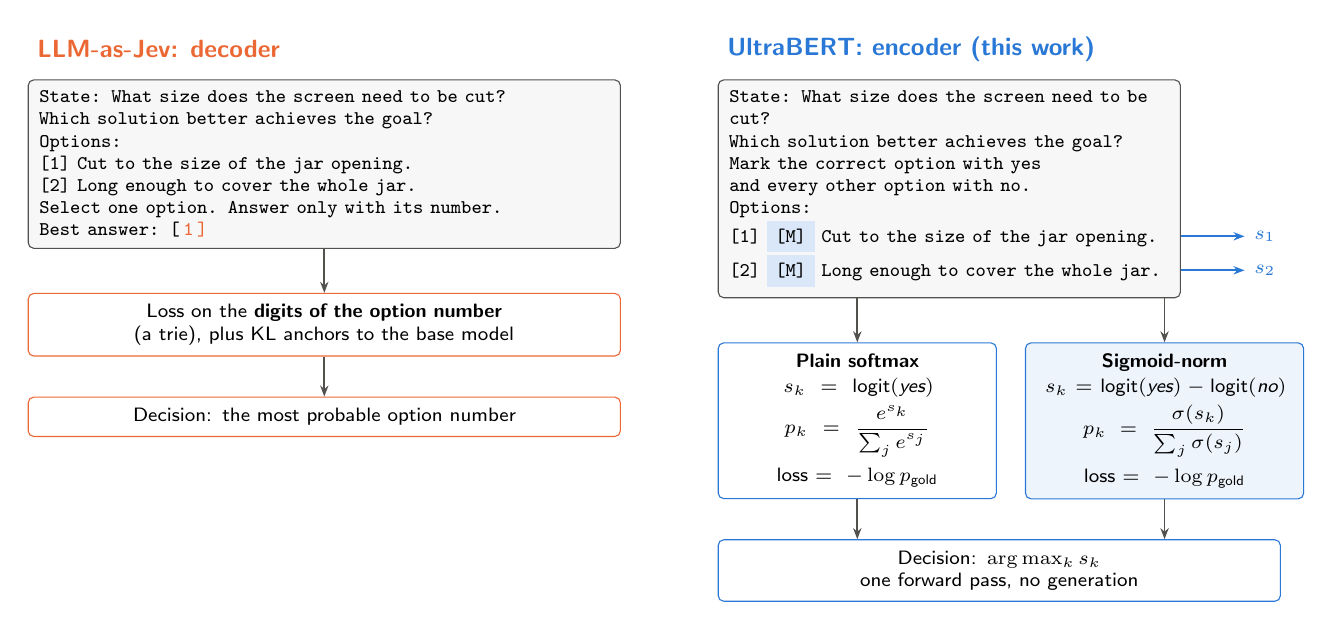
\begin{tikzpicture}[x=1in, y=1in,
      font=\sffamily\scriptsize,
      prompt/.style={draw=ink2, line width=0.4pt, rounded corners=2pt, fill=black!3, inner sep=4pt,
                     align=left, font=\ttfamily\scriptsize},
      box/.style={draw, rounded corners=2pt, inner sep=4pt, align=center, text width=2.85in},
      arr/.style={-{Stealth[length=4pt]}, line width=0.6pt, color=ink2},
      head/.style={font=\sffamily\bfseries\small, anchor=west}]
    % ---------------- decoder (left) ----------------
    \node[head, text=decoder] at (0, 0) {LLM-as-Jev: decoder};
    \node[prompt, text width=2.85in, anchor=north west] (dp) at (0, -0.15) {%
      State: What size does the screen need to be cut?\\
      Which solution better achieves the goal?\\
      Options:\\
      \relax[1] Cut to the size of the jar opening.\\
      \relax[2] Long enough to cover the whole jar.\\
      Select one option. Answer only with its number.\\
      \textbf{Best answer:} \relax[\,\textcolor{decoder}{\textbf{1\,]}}};
    \node[box, draw=decoder, below=0.22in of dp] (dt) {Loss on the \textbf{digits of the option number}\\
      (a trie), plus KL anchors to the base model};
    \node[box, draw=decoder, below=0.2in of dt] (dd) {Decision: the most probable option number};
    \draw[arr] (dp) -- (dt);  \draw[arr] (dt) -- (dd);
    % ---------------- encoder (right) ----------------
    \node[head, text=encoder] at (3.45, 0) {UltraBERT: encoder (this work)};
    \node[prompt, text width=2.2in, anchor=north west] (ep) at (3.45, -0.15) {%
      State: What size does the screen need to be cut?\\
      Which solution better achieves the goal?\\
      Mark the correct option with yes\\and every other option with no.\\
      Options:\\
      \relax[1] \colorbox{encoder!18}{[M]} Cut to the size of the jar opening.\\
      \relax[2] \colorbox{encoder!18}{[M]} Long enough to cover the whole jar.};
    \node[align=left, text=encoder] (s1) at ($(ep.south east)+(0.42in, 0.31in)$) {$s_1$};
    \node[align=left, text=encoder] (s2) at ($(ep.south east)+(0.42in, 0.14in)$) {$s_2$};
    \draw[arr, color=encoder] ($(ep.south east)+(0, 0.31in)$) -- (s1);
    \draw[arr, color=encoder] ($(ep.south east)+(0, 0.14in)$) -- (s2);
    \node[box, draw=encoder, text width=1.28in, anchor=north west] (sm) at ($(ep.south west)+(0,-0.22in)$) {%
      \textbf{Plain softmax}\\[1pt]
      $s_k=\text{logit}(\textit{yes})$\\[2pt]
      $p_k=\dfrac{e^{s_k}}{\sum_j e^{s_j}}$\\[3pt]
      loss $=-\log p_{\text{gold}}$};
    \node[box, draw=encoder, fill=encoder!8, text width=1.28in, anchor=north west] (sg) at ($(sm.north east)+(0.14in,0)$) {%
      \textbf{Sigmoid-norm}\\[1pt]
      $s_k=\text{logit}(\textit{yes})-\text{logit}(\textit{no})$\\[2pt]
      $p_k=\dfrac{\sigma(s_k)}{\sum_j\sigma(s_j)}$\\[3pt]
      loss $=-\log p_{\text{gold}}$};
    \node[box, draw=encoder, text width=2.7in, anchor=north west] (ed) at ($(sm.south west)+(0,-0.2in)$) {Decision: $\arg\max_k s_k$\\one forward pass, no generation};
    \draw[arr] ($(sm.north)+(0,0.22in)$) -- (sm.north);
    \draw[arr] ($(sg.north)+(0,0.22in)$) -- (sg.north);
    \draw[arr] (sm.south) -- (sm.south |- ed.north);
    \draw[arr] (sg.south) -- (sg.south |- ed.north);
  \end{tikzpicture}
  \caption{One row, two ways. The decoder reads the numbered options and writes the number of its answer; the
  loss is taken over the tokens of that number. The encoder gets a mask in front of each option and scores each
  option directly. Two of the three recipes are shown: the plain softmax over the options, which scores an
  option by the ``yes'' logit alone, and the sigmoid-normalised loss, which scores it by ``yes'' minus ``no''.
  Each option's score goes through a sigmoid, and the sum in the denominator keeps the options competing. The third recipe is the softmax over ``yes'' minus ``no''.}
  \label{fig:intro}
\end{figure}


\subsection{Loss functions}
\label{sec:loss}

\paragraph{Decoder: trie loss with KL anchors.}
At each node of the trie the model chooses among the tokens that are legal there.
The tree loss is the negative log-probability of the gold option, which is the product of the choices along its path, each normalised over the legal tokens only,
\begin{equation}
  \mathcal{L}_{\text{tree}} = -\sum_{t}\log\frac{\exp z_t(g_t)}{\sum_{v\in\mathcal{V}_t}\exp z_t(v)},
\end{equation}
where $z_t$ are the logits at step $t$, $g_t$ the gold token and $\mathcal{V}_t$ the legal tokens.
Three anchor terms keep the model close to its starting version $p_0$ \citep{li2026llmasjev}: $\mathcal{L}_{\text{mass}}$ keeps the total probability on the legal tokens, $\mathcal{L}_{\text{out}}$ keeps how the remaining probability is spread over the rest of the vocabulary, and $\mathcal{L}_{\text{pos}}$ keeps the next-token distribution at the start of the reply and after the closing bracket.
They are KL divergences to $p_0$, computed over its 64 most likely tokens and one bucket for the rest.
The loss is $\mathcal{L}=\mathcal{L}_{\text{tree}}+\lambda\,(\mathcal{L}_{\text{mass}}+\mathcal{L}_{\text{out}}+\mathcal{L}_{\text{pos}})$ with $\lambda=1$.

\paragraph{Encoder recipes.}
Let $\ell_k(v)$ be the logit of token $v$ at mask $k$, and let $g$ be the gold option.
A score $s_k$ says how strongly the model accepts option $k$; the decision is the option with the highest score.
Training raises the gold option's score relative to the other options, but no mask gets its own yes-or-no target.
Thus, a chosen option can still prefer ``no'': for example, scores of $-3$ and $-8$ select the first option.
We train the following four recipes:
\begin{itemize}
  \item \textbf{Yes-logit softmax.}
    The score is the ``yes'' logit alone, and the options compete through one softmax:
    \begin{equation}
      s_k=\ell_k(\textit{yes}),\qquad
      p_k=\frac{e^{s_k}}{\sum_{j=1}^{K}e^{s_j}},\qquad
      \mathcal{L}_{\text{softmax}}=-\log p_g.
    \end{equation}

  \item \textbf{Yes-minus-no softmax.}
    The score measures the preference for ``yes'' over ``no'', followed by the same softmax:
    \begin{equation}
      s_k=\ell_k(\textit{yes})-\ell_k(\textit{no}),\qquad
      p_k=\frac{e^{s_k}}{\sum_{j=1}^{K}e^{s_j}},\qquad
      \mathcal{L}_{\text{softmax}}=-\log p_g.
    \end{equation}

  \item \textbf{Yes-minus-no sigmoid normalisation.}
    Each score first goes through a sigmoid, and the resulting values are normalised by their sum:
    \begin{equation}
      s_k=\ell_k(\textit{yes})-\ell_k(\textit{no}),\qquad
      p_k=\frac{\sigma(s_k)}{\sum_{j=1}^{K}\sigma(s_j)},\qquad
      \mathcal{L}_{\text{sig-norm}}=-\log p_g.
    \end{equation}
    This has the form of the DeepSeek-V3 mixture-of-experts gate \citep{deepseekv3}, but the options play the role of experts and are normalised over all $K$ options, with no selection or balancing bias.
    Each $\sigma(s_k)$ lies between 0 and 1 and can be read as how strongly the model accepts option $k$ on its own, although only the ratios enter $p_k$.
    The options therefore still compete, and the decision remains the option with the highest score because the sigmoid is increasing.
    The gradient with respect to $s_k$ is
    \begin{equation}
      \left(1-\sigma(s_k)\right)
      \left(p_k-\mathbf{1}[k=g]\right).
    \end{equation}
    Once an option's sigmoid is close to 1, its score hardly changes.
    We do not pair this normalisation with the ``yes'' logit alone: vocabulary logits are around 200 (\cref{sec:precision}), so every sigmoid is close to 1, every option receives probability $1/K$, and the gradient is negligible.
    The ``yes''-minus-``no'' score is much smaller and avoids this saturation.
    Nothing in the loss makes $\sigma(s_k)$ a probability that holds on its own; \cref{sec:coupling} checks what the trained model does.

  \item \textbf{Yes-minus-no square-root softplus.}
    To test whether the sigmoid's upper bound matters, we use
    $h(s)=\sqrt{\log(1+e^s)}$:
    \begin{equation}
      s_k=\ell_k(\textit{yes})-\ell_k(\textit{no}),\qquad
      p_k=\frac{h(s_k)}{\sum_{j=1}^{K}h(s_j)},\qquad
      \mathcal{L}_{\text{sqrt-sp}}=-\log p_g.
    \end{equation}
    For a clearly rejected option ($s\ll0$), $h(s)\approx e^{s/2}$, so the options behave as in a softmax at twice the temperature.
    For a clearly accepted option ($s\gg0$), $h(s)\approx\sqrt{s}$ keeps growing, whereas the sigmoid stops at 1.
    Its score therefore continues to receive a small gradient where the sigmoid would receive almost none.
\end{itemize}

\section{Experimental setup}
\label{sec:setup}

\subsection{Training data}
\label{sec:data}

We follow LLM-as-Jev \citep{li2026llmasjev} and train on its Reason+Long mixture, with Nimble added.
It has 13 datasets: intent routing (CLINC150, MASSIVE, Bitext), short reasoning (ReClor, LogiQA~2.0, CosmosQA, PIQA, ANLI, ProofWriter), long input (ContractNLI, MuSiQue, QuALITY) and Nimble.
Each is turned into a state (the passages), a question and a list of options.
We keep \NPerDataset{} training rows per dataset, \NTrain{} in total.
Rows are filtered in this order:
\begin{enumerate}\setlength{\itemsep}{0pt}\setlength{\topsep}{2pt}
  \item \textbf{Duplicates.} Rows with the same input are collapsed to one, and rows with the same input but different answers are removed.
  \item \textbf{Leakage between splits.} A training row is removed if its input, or the source document it comes from, also appears in the validation split.
  \item \textbf{Benchmark overlap.} A training row is removed if it shares a 13-word n-gram, or an identical sentence of six or more words, with any evaluation benchmark.
  \item \textbf{Length.} Prompts longer than \MaxTokens{} tokens are dropped, never truncated.
\end{enumerate}
The held-out rows are drawn from the validation split with the same duplicate and length filters, up to 500 per dataset and in whole source documents, giving \NHeldOut{} rows.
We split them into a dev set of \NDev{} rows, used to choose learning rates, and a test set of \NTest{} rows that no choice depends on.

\subsection{Models}
\label{sec:models}

\paragraph{Encoder.}
UltraBERT-380M \citep{ultrabert} is fully fine-tuned with the format of \cref{sec:format}, once with the plain softmax and once with the sigmoid-normalised loss.

\paragraph{Decoders.}
We train Qwen3-0.6B \citep{qwen3} with the full LLM-as-Jev recipe (trie loss and the three anchors, $\lambda=1$), updating all weights.
The anchors use a frozen copy of the starting model as $p_0$.
We also report two LoRA models \citep{lora} that we trained earlier with the same recipe and released, Qwen3-0.6B and Qwen3-4B.
They reach \TestQwLora{}\% and \TestQwFourLora{}\% on the test set (\cref{tab:headline}).
Full fine-tuning of the 0.6B decoder reaches \TestQwFull{}\%, \DiffQwFullQwLora{} points above LoRA, and the encoder is fully fine-tuned, so full fine-tuning is the matched comparison and the LoRA models are references.
They were trained on the 12K-row release of the data without ReClor, while all new runs use the 13K-row mixture with ReClor.

\subsection{Protocol}
\label{sec:protocol}

Every model is trained for one epoch with a batch of 32 rows.
We sweep the learning rate with one seed per value and choose by accuracy on the dev set:
$\{8\cdot10^{-6}, 1.5\cdot10^{-5}, 3\cdot10^{-5}, 5\cdot10^{-5}\}$ for the encoder with the softmax, $\{8\cdot10^{-6}, 1.5\cdot10^{-5}, 2\cdot10^{-5}, 3\cdot10^{-5}\}$ with the sigmoid-normalised loss, and $\{5\cdot10^{-6}, 10^{-5}, 2\cdot10^{-5}\}$ for the decoder.
The two best Qwen rates differ by 0.1 points on dev, and we use $10^{-5}$.
At the chosen rate we repeat the run with different seeds, which change the order of the rows and the option shuffling, and report the average.
The test set is not used for any of these choices.

The metric is accuracy.
ALL is the mean accuracy over the 13 datasets, so that every dataset counts equally.
On the test set we average each row's correctness over the seeds of a model and report ALL of this average.
The encoder is scored with fp32 weights under bf16 autocast, because bf16 weights change its long-document results.
The Qwen checkpoints are scored with bf16 weights, as the released models are.

\subsection{External benchmarks and cost}
\label{sec:external}

To see whether training on the mixture changes behaviour outside it, we score six benchmarks as decision rows: BoolQ, MMLU, MMLU-Pro, ARC-Challenge, Winogrande and SciQ, with 500, 1200, 800, 600, 500 and 400 rows.
The sample sizes follow LLM-as-Jev, whose samples are not released, so ours are seeded uniform draws.
External is the mean accuracy over the six.
These benchmarks are not used for any choice.

Time per decision is the mean over 1{,}300 held-out rows on one A100, with one row at a time.

\section{Results}
\label{sec:results}

\subsection{Encoder against decoder}

\Cref{tab:headline} and \cref{fig:headline} give the main comparison.
With the same data and training budget, every encoder recipe is above Qwen3-0.6B (\TestQwFull{}\% on the test set): \TestUbList{}\% with the softmax over ``yes'', and \TestUbYesNo{}\%, \TestUbSqrt{}\% and \TestUbSig{}\% with the softmax, the square-root softplus and the sigmoid over ``yes'' minus ``no''.
The encoder also has fewer parameters, 380M against 0.6B.
On the six external benchmarks the encoder recipes reach \ExtUbList{}\% to \ExtUbYesNo{}\%, against \ExtQwFull{}\% for the decoder.
The reproduced Qwen3-4B LoRA model, at \TestQwFourLora{}\%, remains ahead of all sub-billion models, so our claims are limited to models below one billion parameters.

\subsection{Full fine-tuning against LoRA}

The reproduced LoRA model of the same size reaches \TestQwLora{}\%, \DiffQwFullQwLoraAbs{} points below the fully fine-tuned decoder.
Both were trained on the same data, so this gap comes from updating all weights instead of a LoRA adapter, and accounts for about half of the \DiffUbSigQwLoraText{}-point gap between the best encoder recipe and the LoRA model.
The external accuracy of fully fine-tuned Qwen3-0.6B (\ExtQwFull{}\%) is not above that of its LoRA model (\ExtQwLora{}\%).

\subsection{Recipes}

Scoring by ``yes'' minus ``no'' gives most of the gain: over the ``yes'' logit alone it adds \DiffUbYesNoUbListAbs{} points on the test set and \ExtUbYesNo{}\% against \ExtUbList{}\% on the external benchmarks.
The sigmoid normalisation adds a further \DiffUbSigUbYesNoAbs{} points on the test set and nothing on the external benchmarks, and its results vary less between seeds.
The square-root softplus works like the sigmoid but has no upper bound, and it does no better than the softmax (\TestUbSqrt{}\% against \TestUbYesNo{}\%).
This suggests that the bound of the sigmoid is what helps.
The bound is not the only difference, though: for rejected options the square-root softplus also acts as a softmax at twice the temperature (\cref{sec:loss}).
\Cref{sec:analysis} compares the labels that each recipe predicts.

\subsection{How strongly the options depend on each other}
\label{sec:coupling}

In a softmax, raising one option's score lowers the probability of every other option, so the options are tied together.
DeepSeek-V3 gates its experts with a sigmoid instead \citep{deepseekv3}.
We test whether the normalisation changes how much the answer depends on the other options.
On the dev rows we shuffle the options four times and remove one wrong option, and count how often the answer changes (\cref{tab:coupling}).
Comparing the two softmax recipes shows the effect of the score; comparing the softmax and the sigmoid over ``yes'' minus ``no'' shows the effect of the normalisation.

The score does most of the work: ``yes'' minus ``no'' raises external accuracy from \CpExtYes{}\% to \CpExtYesNo{}\%, lowers the answer changes when a wrong option is removed from \CpDropYes{}\% to \CpDropYesNo{}\%, and lowers the largest gradient norm from \CpGradYes{} to \CpGradYesNo{}.
When the options are shuffled, the score and the sigmoid each lower the answer changes by about one point (\CpShufYes{}\%, \CpShufYesNo{}\%, \CpShufSig{}\%).
On top of the score, the sigmoid raises dev accuracy from \CpAccYesNo{}\% to \CpAccSig{}\%, lowers the calibration error from \CpEceYesNo{} to \CpEceSig{}, and brings the share of each predicted label closer to its share among the gold answers, which the score alone moves further away (total variation \CpLabelYes{}, \CpLabelYesNo{}, \CpLabelSig{}).
After training, the gold option's sigmoid averages only \CpSigGoldSig{}; far below 1, $\sigma(s)\approx e^{s}$, so the loss behaves almost like a softmax.
The square-root softplus has the smallest gradient spikes in training (largest norm \CpGradSqrt{}), but it changes its answer most often when the options are shuffled (\CpShufSqrt{}\%).

\subsection{Cost}

The encoder takes \MsUb{}\,ms per decision on one A100, one row at a time, against \MsQwFull{}\,ms for Qwen3-0.6B and \MsQwFourLora{}\,ms for Qwen3-4B.
\Cref{app:impl} gives the batched throughput.

\begin{table}[t]
  \centering\small
  \caption{Matched comparison: average accuracy (\%) over seeds. Test ALL is on the test set;
  Dev ALL and External are on the dev set and the six external benchmarks. Learning rates were chosen on
  dev. Bold: best below 1B parameters.}
  \label{tab:headline}
  % Generated by paper/figures/make_figures.py; do not edit.
\begin{tabular}{@{}llccc@{}}
\toprule
Model & Params & Dev ALL & Test ALL & External \\
\midrule
UltraBERT-380M, sigmoid\_norm & 380M & 72.7 & \textbf{72.1} & 59.5 \\
UltraBERT-380M, listwise & 380M & 71.2 & 69.7 & 57.8 \\
Qwen3-0.6B, full FT & 0.6B & 69.0 & 67.6 & 56.1 \\
Qwen3-0.6B, LoRA (released) & 0.6B & 64.5 & 63.0 & 56.9 \\
\midrule
Qwen3-4B, LoRA (released) & 4B & 79.3 & 77.3 & 73.5 \\
\bottomrule
\end{tabular}

\end{table}

\begin{figure}[t]
  \centering
  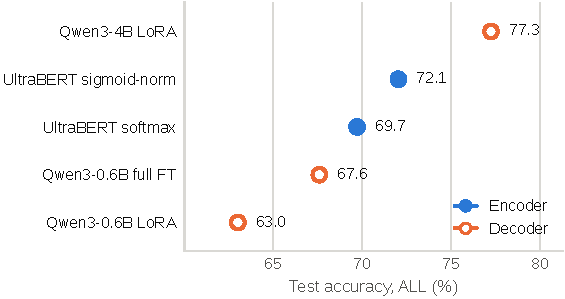
\includegraphics[width=0.62\linewidth]{fig_headline}
  \caption{Test accuracy (ALL, the mean over 13 datasets, on the test set, never used for any choice),
  averaged over seeds; \textcolor{encoder}{encoders} filled, \textcolor{decoder}{decoders} hollow.}
  \label{fig:headline}
\end{figure}

\begin{table}[t]
  \centering\small
  \caption{How strongly the options depend on each other, on the dev set (average scores). Each row is scored in four
  random option orders and once with one wrong option removed. TV: total variation between the predicted and the gold shares,
  over the three datasets with a fixed label set (label) and over option positions (position); lower is closer.
  Calibration error: expected calibration error of the top option's probability. $|s_k|$: size of the raw option scores. Bold: best in each row; accuracy is better higher, the other scores lower.}
  \label{tab:coupling}
  % Generated by paper/figures/make_figures.py; do not edit.
\begin{tabular}{@{}lccc@{}}
\toprule
& \begin{tabular}[b]{@{}c@{}}Softmax,\\``yes''\end{tabular} & \begin{tabular}[b]{@{}c@{}}Softmax,\\``yes'' $-$ ``no''\end{tabular} & \begin{tabular}[b]{@{}c@{}}Sigmoid-norm,\\``yes'' $-$ ``no''\end{tabular} \\
\midrule
Dev accuracy (\%) & 71.4 & 71.5 & \textbf{72.9} \\
\midrule
Answer changes, options shuffled (\%) & 15.6 & \textbf{12.7} & 13.7 \\
Answer changes, one wrong option removed (\%) & 5.9 & \textbf{4.3} & 4.9 \\
Largest gradient norm in training & 842 & 226 & \textbf{190} \\
\midrule
Label shares vs.\ gold (TV) & 0.167 & 0.219 & \textbf{0.139} \\
Position shares vs.\ gold (TV) & 0.050 & 0.048 & \textbf{0.041} \\
Calibration error, top option & 0.038 & 0.030 & \textbf{0.023} \\
Mean $|s_k|$ & 60.5 & 3.1 & 7.4 \\
\bottomrule
\end{tabular}

\end{table}

\section{Analysis}
\label{sec:analysis}

This section describes what we saw when training UltraBERT.
Unless noted, the numbers are from the dev set with one seed per setting.

\subsection{Learning rate and training length}

The learning rate that is best on dev, $1.5\cdot10^{-5}$ for both swept recipes, is also among the best on the external benchmarks.
Higher rates add little on dev and lower the external accuracy, down to 53.2\% for the softmax at $5\cdot10^{-5}$.
Qwen3-0.6B shows the same pattern more strongly: its external accuracy falls with every increase of the rate, from 57.4\% at $5\cdot10^{-6}$ to 53.9\% at $2\cdot10^{-5}$.
A second epoch has the same effect.
With the softmax at $3\cdot10^{-5}$ it raises dev accuracy from 70.7\% to 73.9\%, above any one-epoch encoder run, and lowers external accuracy from 56.2\% to 55.1\%.
We report one epoch for all models, since a longer run fits the mixture at the cost of behaviour outside it.

\subsection{Datasets}

\Cref{tab:perdataset} in the appendix gives the test accuracy for every dataset, averaged over seeds.
The sigmoid-normalised encoder is above the fully fine-tuned decoder on 10 of the 13 datasets.
The gaps are largest on CosmosQA, ANLI and QuALITY, where it is ahead by 15.3, 9.9 and 9.8 points, and on MASSIVE (8.0) and MuSiQue (6.9).
It is below the decoder on three datasets: Nimble ($-6.6$), LogiQA~2.0 ($-2.2$) and ProofWriter ($-1.7$).
The 4B decoder is ahead of the encoder on all ten datasets outside intent routing.
The gap is 12 to 19 points on ReClor, Nimble and LogiQA~2.0, and below one point on CosmosQA, ANLI and ContractNLI.
On the three intent datasets, CLINC150, MASSIVE and Bitext, the encoder is level with or slightly above the 4B decoder, by 1.4 to 2.1 points.

\subsection{Loss and score}

\Cref{tab:ablation} separates the changes between the plain softmax and the sigmoid-normalised loss.
Scoring with the difference of the ``yes'' and ``no'' logits, with the softmax kept, raises the external accuracy by 2.0 points and the dev accuracy by 0.4 points; averaged over seeds, the score accounts for the whole external gain (\CpExtYes{}\%, \CpExtYesNo{}\%, \CpExtSig{}\% in \cref{tab:coupling}).
Replacing the softmax with the sigmoid-normalised loss then raises dev accuracy by a further 1.3 points, and MuSiQue most of all, from 64\% to 76\%.
Nimble falls from 55\% with the plain score to 43\% with the sigmoid-normalised loss in this one run, on 100 dev rows.
On the test set, averaged over seeds, the sigmoid-normalised model is instead 3.7 points above the softmax on Nimble.
Replacing ``yes'' with ``correct'' did not help in this run: 70.6\% against 71.1\% with the ``yes'' logit, and 70.1\% against 71.5\% for the difference with ``incorrect''.

The recipes also predict different labels.
On MuSiQue the correct answer is ``Yes'' in 48\% of the rows.
The sigmoid-normalised models predict ``Yes'' for 47 to 60\% of the rows, against 64\% and 69\% for the two softmax variants (dev rows).
On ProofWriter, where ``Unknown'' is correct for a third of the rows, the softmax never predicts it and the sigmoid-normalised models predict it for 2 to 12\%.
This class stays largely unlearned for every variant.

\begin{table}[t]
  \centering\small
  \caption{Encoder variants on the dev rows, one seed (accuracy, \%). The first row is the softmax with the ``yes'' logit,
  the setting used for the softmax results elsewhere. Bold: best in each column.}
  \label{tab:ablation}
  % Generated by paper/figures/make_figures.py; do not edit.
\begin{tabular}{@{}lccccc@{}}
\toprule
Variant & Dev ALL & External & MuSiQue & ContractNLI & Nimble \\
\midrule
Softmax, ``yes'' & 71.1 & 57.1 & 57.0 & 75.0 & 55.0 \\
Softmax, ``yes'' $-$ ``no'' & 71.5 & 59.1 & 64.0 & 78.0 & 48.0 \\
Sigmoid-norm, ``yes'' $-$ ``no'' & 72.8 & 59.4 & 76.0 & 81.0 & 43.0 \\
Softmax, ``correct'' & 70.6 & 56.8 & 48.0 & 77.0 & 52.0 \\
Softmax, ``correct'' $-$ ``incorrect'' & 70.1 & 58.0 & 54.0 & 76.0 & 46.0 \\
\bottomrule
\end{tabular}

\end{table}

\subsection{Numerical precision}
\label{sec:precision}

The encoder has to be scored with fp32 weights under bf16 autocast.
Its masked-token logits are of the order of 200, where bf16 can only step by 1 or 2, so options tie or swap.
With bf16 weights the MuSiQue accuracy drifts by up to 8 points.
The decoders are scored with bf16 weights, and re-scoring a Qwen checkpoint in another precision moved its dev accuracy by at most 0.8 points.

\section{Citing the evidence}
\label{sec:citation}

A decision model writes no text, so it gives no reasons for its choice.
We add a small evidence head that marks the sentences of the document that support the chosen option.
Because the encoder reads the question, the options and the document together, the hidden state of every document token already depends on all of them, and a head on top of these states can score the tokens.
The encoder stays frozen, so its decisions do not change, and one forward pass gives the decision and the evidence.
For each document token, the head reads the token's hidden state and the hidden state at the mask of the chosen option, and outputs the probability that the token supports that option.
The score of a sentence is the highest probability among its tokens.

The head is trained on evidence labels.
Where a dataset has human-marked evidence we use it, and for the other datasets we generate it with the SelfCite necessity and sufficiency reward \citep{selfcite}, as \cref{fig:spans} shows.
A labelling model proposes several sets of sentences as evidence for the gold answer.
We then score each set on the decision prompt, with the set removed and with only the set kept, and keep the set with the highest reward.
\Cref{app:evidence} gives the details.

% Figure: how the evidence labels are generated (best-of-N with the SelfCite reward). Settings = span_generation/best_of_n.py defaults.
\begin{figure}[t]
  \centering
  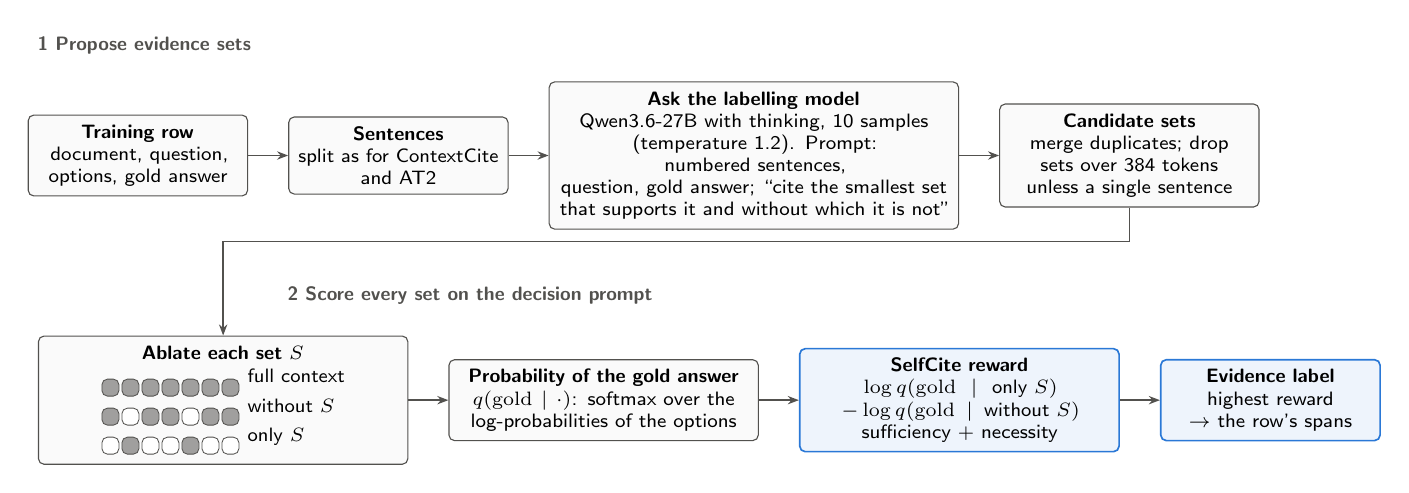
\begin{tikzpicture}[x=1in, y=1in,
      font=\sffamily\scriptsize,
      box/.style={draw=ink2, line width=0.4pt, rounded corners=2pt, inner sep=3.5pt, align=center, fill=black!2},
      key/.style={draw=encoder, line width=0.6pt, rounded corners=2pt, inner sep=3.5pt, align=center, fill=encoder!8},
      arr/.style={-{Stealth[length=4pt]}, line width=0.6pt, color=ink2},
      lane/.style={font=\sffamily\bfseries\scriptsize, text=ink2, anchor=west},
      sq/.style={draw=ink2, line width=0.3pt, minimum size=0.085in, inner sep=0pt}]
    % ------------- lane 1: propose -------------
    \node[lane] at (0, 0.2) {1  Propose evidence sets};
    \node[box, text width=1.0in] (row) at (0.55, -0.35) {\textbf{Training row}\\document, question,\\options, gold answer};
    \node[box, text width=1.0in, right=0.2in of row] (sent) {\textbf{Sentences}\\split as for ContextCite\\and AT2};
    \node[box, text width=1.95in, right=0.2in of sent] (ask) {\textbf{Ask the labelling model}\\Qwen3.6-27B with thinking, 10 samples\\(temperature 1.2). Prompt: numbered sentences,\\question, gold answer; ``cite the smallest set\\that supports it and without which it is not''};
    \node[box, text width=1.2in, right=0.2in of ask] (cand) {\textbf{Candidate sets}\\merge duplicates; drop\\sets over 384 tokens\\unless a single sentence};
    \draw[arr] (row) -- (sent); \draw[arr] (sent) -- (ask); \draw[arr] (ask) -- (cand);
    % ------------- lane 2: score -------------
    \node[lane] at (1.25, -1.05) {2  Score every set on the decision prompt};
    \node[box, text width=1.75in, anchor=north west] (abl) at (0.05, -1.25) {%
      \textbf{Ablate each set $S$}\\[2pt]
      \begin{tabular}{@{}l@{\hspace{3pt}}l@{}}
        \tikz[baseline=-0.5ex]{\foreach \i/\c in {1/ink2!55,2/ink2!55,3/ink2!55,4/ink2!55,5/ink2!55,6/ink2!55,7/ink2!55}{\node[sq, fill=\c] at (\i*0.1, 0) {};}} & full context \\[1pt]
        \tikz[baseline=-0.5ex]{\foreach \i/\c in {1/ink2!55,2/white,3/ink2!55,4/ink2!55,5/white,6/ink2!55,7/ink2!55}{\node[sq, fill=\c] at (\i*0.1, 0) {};}} & without $S$ \\[1pt]
        \tikz[baseline=-0.5ex]{\foreach \i/\c in {1/white,2/ink2!55,3/white,4/white,5/ink2!55,6/white,7/white}{\node[sq, fill=\c] at (\i*0.1, 0) {};}} & only $S$
      \end{tabular}};
    \node[box, text width=1.45in, right=0.2in of abl] (q) {\textbf{Probability of the gold answer}\\$q(\mathrm{gold}\mid\cdot)$: softmax over the\\log-probabilities of the options};
    \node[key, text width=1.5in, right=0.2in of q] (rew) {\textbf{SelfCite reward}\\$\log q(\mathrm{gold}\mid\text{only }S)$\\$-\log q(\mathrm{gold}\mid\text{without }S)$\\sufficiency + necessity};
    \node[key, text width=1.0in, right=0.2in of rew] (out) {\textbf{Evidence label}\\highest reward\\$\to$ the row's spans};
    \draw[arr] (cand.south) -- ++(0, -0.17) -| (abl.north);
    \draw[arr] (abl) -- (q); \draw[arr] (q) -- (rew); \draw[arr] (rew) -- (out);
  \end{tikzpicture}
  \caption{How evidence labels are generated for rows without human evidence. A labelling model proposes sets of
  sentences as evidence for the \emph{gold} answer. Each set $S$ is scored on the decision prompt by removing it and by
  keeping only it: a good set is enough to keep the answer (sufficiency) and its removal loses the answer (necessity).
  The set with the highest reward becomes the label, which trains the evidence head. Unlike SelfCite, the answer scored is
  the gold answer and not the model's own response.}
  \label{fig:spans}
\end{figure}


\paragraph{Comparison.}
We compare the head with three methods that score the sentences of the document for a given decision: the average attention of the encoder, AT2 \citep{at2} and ContextCite \citep{contextcite}.
The test rows are 200 held-out rows with gold evidence, 50 each from ContractNLI, MuSiQue, Nimble and ProofWriter.
Each method is conditioned on the option that the model chooses.
We report the average precision of the sentence ranking against the gold sentences, and how often the top sentence is gold.
For the three baselines we also report the faithfulness score LDS, the rank correlation between the predicted and the actual change in the probability of the answer when random sets of sentences are removed, and for all methods the time per row.
AT2 and ContextCite were run on the encoder trained with the softmax, so \cref{tab:citation} has a head for that encoder, as well as one for the encoder trained with the sigmoid-normalised loss.

\begin{table}[t]
  \centering\small
  \caption{Sentence evidence on 200 held-out rows with gold evidence. Sentence AP: average precision against the gold
  sentences. Top-1: share of rows where the top sentence is gold. LDS: faithfulness to the model, defined for the
  three methods that explain it. The first three methods and the first head use the encoder trained with the softmax.}
  \label{tab:citation}
  % Generated by paper/figures/make_figures.py; do not edit.
\begin{tabular}{@{}lcccccccc@{}}
\toprule
& \multicolumn{5}{c}{Sentence AP} & & & \\
\cmidrule(lr){2-6}
Method & All & CNLI & MuSiQue & Nimble & PW & Top-1 (\%) & LDS & ms per row \\
\midrule
Average attention & 0.26 & 0.08 & 0.19 & 0.40 & 0.37 & 15 & 0.11 & \textbf{42} \\
AT2 & 0.33 & 0.34 & 0.29 & 0.30 & 0.39 & 22 & 0.18 & 47 \\
ContextCite & 0.41 & 0.54 & 0.34 & 0.33 & 0.41 & 45 & \textbf{0.65} & 1{,}704 \\
\midrule
Evidence head, softmax encoder & 0.56 & 0.28 & 0.32 & \textbf{0.97} & \textbf{0.68} & 56 & -- & 67 \\
Evidence head, sigmoid-norm encoder & \textbf{0.68} & \textbf{0.56} & \textbf{0.50} & \textbf{0.97} & \textbf{0.68} & \textbf{74} & -- & 75 \\
\bottomrule
\end{tabular}

\end{table}

\paragraph{Results.}
On the same encoder, the head has a higher sentence AP than ContextCite and AT2 (\EvSentAPList{} against \ContextCiteSentAP{} and \AtTwoSentAP{}), and its top sentence is gold more often (\EvTopOneList{}\% against \ContextCiteTopOne{}\% and \AtTwoTopOne{}\%).
It does so in \EvMsList{}\,ms, against \ContextCiteMs{}\,ms for ContextCite, which needs a forward pass for each of many ablations.
AT2 is as fast, at \AtTwoMs{}\,ms, and has a lower sentence AP.
The head on the encoder trained with the sigmoid-normalised loss is better again, with a sentence AP of \EvSentAPSig{}, \EvTopOneSig{}\% for the top sentence and \EvMsSig{}\,ms per row.
At the token level its average precision is \EvTokAPSig{}, against \EvChanceSig{} for a random ranking, and the precision of its ten highest tokens is \EvPTenSig{}.
The words that it marks with the tuned threshold of \EvThrSig{} have a precision of \EvWordPSig{} and a recall of \EvWordRSig{}, so the marked words are a rough guide and not an exact span.

The accuracy of the evidence depends on the dataset.
For the head on the sigmoid-normalised encoder, the sentence AP is 0.97 on Nimble and 0.68 on ProofWriter, and 0.56 on ContractNLI and 0.50 on MuSiQue, where the documents are long and the gold sentences few.

\paragraph{What the head does not show.}
ContextCite is the most faithful to the model, with an LDS of \ContextCiteLds{}, against \AtTwoLds{} for AT2.
The head has no LDS, because it is trained to predict the evidence that an annotator would mark, and not what the model used.
It is a pointer to the support for the answer, and it gives no proof that the model used it.
The comparison is also not between equals: the head is trained on labels from the same datasets, while ContextCite uses no labels.

\section{Related work}
\label{sec:related}

\paragraph{Jev-style decision models.}
Most of the community decision models compared in LLM-as-Jev \citep{li2026llmasjev} use a decoder backbone and read the logits of an option letter or label, with the backbone frozen or tuned with LoRA.
LLM-as-Jev studies this readout and when fine-tuning helps.
AnyJev reads a typed decision from one prefill and corrects the label prior and the effect of option order without training \citep{zhang2026anyjev}.
The Contrastive Language Model \citep{kwok2026clm} embeds the state (the context and the question) and each candidate separately, with a frozen Qwen3-8B and two projection heads, and scores them by cosine similarity, so the candidate embeddings can be cached.
Because the two are encoded apart, a candidate never attends to the context, and its training starts from tens of millions of pairs.
All of these start from a decoder.
We start from an encoder that reads the context, the question and all options together, and compare the two under the same training data.

\paragraph{Encoders that score options.}
Prompt-based classifiers use the masked-token head of an encoder with a verbalizer for a fixed set of labels \citep{schick2021pet, gao2021lmbff}.
Two encoder decision models are listed on public Jev leaderboards \citep{jevbench}: Laya \citep{laya} and Von \citep{von}, both built on ModernBERT-large with one mask per option.
Both add new layers on top of the encoder, and they are described in model cards.
Laya trains its head with reinforcement learning on proper scoring rules, and Von uses a listwise softmax loss with a Brier term.
We reuse the pretrained masked-token head and score each option by ``yes'' against ``no'', so there is no new head.
We also compare three training recipes, match the decoders in data and training, report a held-out test split, and add evidence.

\paragraph{Option letters, position and label bias.}
Reading the letter of the chosen option requires a model to bind the letter to the option text \citep{robinson2023mcsb}.
Models favour certain option labels, and their accuracy changes when the options are reordered \citep{zheng2024notrobust, pezeshkpour2024order}.
Corrections are usually applied after training, by calibrating with a content-free input \citep{zhao2021calibrate} or by dividing out a label prior and averaging over rotations of the options \citep{zhang2026anyjev}.
We shuffle the options during training and measure how the recipes differ in the labels they predict.

\paragraph{Encoders and decoders.}
Controlled studies pretrain encoders and decoders with the same recipe, and find that encoders do well on classification and retrieval \citep{weller2025ettin} and that masked language modelling suits tasks that need text representations \citep{gisserotboukhlef2025mlm}.
A much larger decoder can still beat an encoder on classification \citep{zhao2024classification}.
Decoder designs such as multi-query and grouped-query attention target long generation \citep{mqa, gqa}, and \citet{prefillonly} study what they cost when nothing is generated (\cref{sec:intro}).
Modern encoders keep long inputs and fast inference \citep{modernbert, ultrabert}.

\paragraph{Attribution and evidence.}
ContextCite learns a surrogate model from many ablations of the context \citep{contextcite}.
AT2 learns to weight attention heads, and needs a decoder pass \citep{at2}.
SelfCite fine-tunes a model to cite, using the change in the answer probability when the cited text is removed or kept alone as the reward \citep{selfcite}.
Rationale benchmarks such as ERASER compare selected evidence with human rationales \citep{deyoung2020eraser}.
We train an evidence head on the encoder with labels from human-marked evidence and from the SelfCite reward, which gives the evidence in one pass.

\section{Conclusion}
\label{sec:conclusion}

We built a decision model on an encoder, UltraBERT-380M, with one mask in front of each option and the model's own ``yes'' versus ``no'' prediction as the score of the option.
With the same data and full fine-tuning, it is more accurate than Qwen3-0.6B trained with LLM-as-Jev (\TestUbSig{}\% against \TestQwFull{}\% on the test set), and takes \MsUb{}\,ms per decision against \MsQwFull{}\,ms.
The sigmoid-normalised loss adds \DiffUbSigUbList{} points over the plain softmax and brings the predicted label rates closer to the true rates on MuSiQue and ProofWriter.
An evidence head on the frozen encoder marks, in the same pass, the sentences an annotator would mark as support. On 200 rows from four datasets it ranks the annotated sentences higher on average than AT2 and ContextCite, which use no evidence labels, though ContextCite is better on two of the four datasets.

The results have limits.
They are at the scale of 0.4 to 0.6 billion parameters, and a 4B decoder is still more accurate overall, except on the intent datasets.
We used one encoder and one training mixture, in English, and compared against one decoder family.
The evidence head predicts the evidence that an annotator would mark, and does not show what the model used; we did not compute its LDS, and ContextCite has the highest LDS of the methods we measured.
We did not measure memory; that argument rests on \citet{prefillonly}.

Two directions follow.
The first is larger encoders, to see whether the advantage holds above one billion parameters.
The second is to train the decision and the evidence together, so that the evidence head can also shape the encoder.


\bibliographystyle{plainnat}
\bibliography{refs}

\appendix
\section{Implementation details}
\label{app:impl}

\Cref{tab:hparams} lists the training settings.
Both models train for one epoch on \NTrain{} rows, which is 406 steps at a batch of 32.

\begin{table}[h]
  \centering\small
  \caption{Training settings. Learning rates are in \cref{sec:protocol}.}
  \label{tab:hparams}
  \begin{tabular}{@{}lll@{}}
    \toprule
    & UltraBERT-380M & Qwen3-0.6B (full) \\
    \midrule
    Optimiser & AdamW, $\beta=(0.9, 0.98)$, $\epsilon=10^{-6}$ & AdamW \\
    Weight decay & 0.1 & 0.01 \\
    Schedule & 5\% warmup, linear decay to 0 & 100 warmup steps, linear decay to 10\% \\
    Gradient clipping & 1.0 & 1.0 \\
    Precision & fp32 weights, bf16 autocast & fp32 weights, bf16 autocast \\
    Attention & FlashAttention-2, varlen & default \\
    Gradient checkpointing & yes & -- \\
    Token limit & 32{,}768 & 16{,}384 \\
    \bottomrule
  \end{tabular}
\end{table}

The encoder settings are those of the UltraBERT model card, and we change only the learning rate.
No training row exceeds either token limit, because the data are cut at \MaxTokens{} tokens (\cref{sec:data}).

\section{Evidence head}
\label{app:evidence}

The evidence head marks the document tokens that support an answer, and runs on top of a frozen encoder.
We train it on a frozen UltraBERT-380M model, so the decisions of the encoder do not change and one forward pass gives both the decision and the evidence.
We train one head on the model fine-tuned with the sigmoid-normalised loss and one on the model fine-tuned with the softmax, both at a learning rate of $1.5\cdot10^{-5}$, because AT2 and ContextCite were run on the softmax model.

\paragraph{Model.}
For document token $t$ and option $k$ the head reads $[h_t;\,h_k;\,h_t\odot h_k]$, where $h_t$ is the final hidden state of the token and $h_k$ that of option $k$'s mask.
Both come from the one forward pass of the encoder, which reads the question and all the options together with the document, so every $h_t$ already depends on them.
A two-layer perceptron with 512 hidden units, GELU and dropout 0.1 maps this vector to one logit, and its sigmoid is the probability that the token is evidence for option $k$.
The score of a sentence is the highest probability among its tokens.

\paragraph{Labels.}
A token is positive if it overlaps an evidence span.
Where a dataset has gold evidence we use it (Nimble, ContractNLI, MuSiQue, ProofWriter).
For rows with no gold evidence we use generated spans, produced as in \cref{fig:spans}.
Qwen3.6-27B, with thinking, is prompted with the numbered sentences of the row, the question and the gold answer, and asked for the smallest set of sentences that supports the answer and without which it is no longer supported.
We sample ten replies at temperature 1.2 and top-$p$ 0.9, merge identical sets, and drop sets that cite more than 384 tokens unless they are a single sentence.
Each remaining set $S$ is scored by the same model on the decision prompt: once with the full context, once without $S$ and once with only $S$, which makes $1+2m$ prompts for $m$ sets.
The score of each option is the sum of the log-probabilities of its tokens, as in the trie of \cref{sec:loss}, and $q(\mathrm{gold}\mid\cdot)$ is the softmax over the options.
The reward of a set is $\log q(\mathrm{gold}\mid\text{only }S)-\log q(\mathrm{gold}\mid\text{without }S)$, the sum of its sufficiency and its necessity with equal weight and no penalty for size, since the token limit already bounds it.
The set with the highest reward is the label of the row.
The labels cover ANLI, QuALITY, LogiQA~2.0, CosmosQA and the rows of ContractNLI, MuSiQue and ProofWriter without gold evidence.
Unlike SelfCite, which scores the model's own response, we score the gold answer, so the reward carries information only where the labelling model believes the gold answer.
We did not check the generated labels against human evidence on their own.
The indirect check is the ablation below: adding them to the gold labels raises the agreement of the head with human evidence.
Gold evidence is used when both exist.
There are 7{,}778 labelled training rows, of which 7{,}390 are used for training and 388 for validation, and 5.2\% of the training tokens are positive.

\paragraph{Training.}
The loss is token-level binary cross-entropy, with the positive class weighted by the ratio of negative to positive tokens (18.1).
In training the head is conditioned on the gold option, and at test time on the option the encoder chooses.
We use AdamW with a learning rate of $10^{-3}$ and weight decay 0.01, 16 rows per step and three epochs, and keep the epoch with the best token average precision on the validation rows.
The encoder stays frozen.

\paragraph{Evaluation.}
We use the 50 rows per dataset, from ContractNLI, MuSiQue, Nimble and ProofWriter, that have gold evidence and at least two sentences, the same rows on which AT2 and ContextCite are scored.
A word is highlighted when its probability is at least a global threshold, the one that gave the best word F1 on 956 other held-out rows: \EvThrSig{} for the head on the sigmoid-normalised model and \EvThrList{} for the head on the softmax model.
Adding the generated labels to the gold ones raises the sentence average precision from \EvSentAPGold{} to \EvSentAPList{} and the token average precision from \EvTokAPGold{} to \EvTokAPList{} (head on the softmax model).

\section{Additional results}
\label{app:extra}

\Cref{tab:perdataset} gives the test accuracy for each dataset, averaged over seeds.

\begin{table}[h]
  \centering\small
  \setlength{\tabcolsep}{4pt}
  \caption{Test accuracy (\%) per dataset, averaged over seeds. UB is UltraBERT-380M. Bold: best below 1B parameters.}
  \label{tab:perdataset}
  % Generated by paper/figures/make_figures.py; do not edit.
\begin{tabular}{@{}lrccccc@{}}
\toprule
Dataset & Rows & UB sig-norm & UB softmax & Qwen full & Qwen LoRA & Qwen-4B LoRA \\
\midrule
CLINC150 & 400 & \textbf{91.8} & \textbf{91.8} & 86.3 & 79.8 & 89.8 \\
MASSIVE & 400 & \textbf{84.9} & 83.7 & 76.9 & 68.8 & 83.5 \\
Bitext & 400 & \textbf{99.3} & \textbf{99.3} & 96.0 & 94.8 & 97.2 \\
\midrule
ReClor & 400 & \textbf{59.9} & 58.9 & 57.7 & 51.2 & 72.2 \\
LogiQA 2.0 & 400 & 54.8 & 52.9 & \textbf{57.0} & 56.0 & 73.5 \\
CosmosQA & 400 & \textbf{75.2} & 74.8 & 59.9 & 55.0 & 76.0 \\
PIQA & 400 & \textbf{75.1} & 74.8 & 70.2 & 68.8 & 83.8 \\
ANLI & 400 & \textbf{73.6} & 73.1 & 63.7 & 61.0 & 74.0 \\
ProofWriter & 400 & 61.6 & 60.7 & \textbf{63.3} & 63.0 & 70.5 \\
\midrule
ContractNLI & 393 & \textbf{78.6} & 73.8 & 76.1 & 65.6 & 79.1 \\
MuSiQue & 400 & \textbf{69.8} & 58.9 & 62.9 & 54.8 & 71.5 \\
QuALITY & 398 & \textbf{61.3} & 56.9 & 51.5 & 50.0 & 68.8 \\
Nimble & 224 & 50.7 & 47.0 & \textbf{57.3} & 50.9 & 64.3 \\
\bottomrule
\end{tabular}

\end{table}

\section{Examples}
\label{app:examples}

The examples show the decision of the sigmoid-normalised encoder and the token scores of its evidence head for one row of each of three datasets.
The rows are the first of each dataset, in the evaluation order of the evidence study, that has at most 1{,}400 tokens; MuSiQue has none.
Only the tokens that the head scores at or above its threshold of \EvThrSig{} for the chosen option are highlighted, darker for a higher probability, and tokens inside the gold evidence are underlined.
The encoder chooses the correct option in all three rows; the rows were picked by the rule above and not by outcome.

% Generated by paper/figures/make_examples.py; do not edit.
\paragraph{ContractNLI.} 1{,}376 tokens.
The model chooses option 1, which is \textbf{correct}. Question: Statement: "Receiving Party may share some Confidential Information with some third-parties (including consultants, agents and professional advisors)." Does the contract entail the statement, contradict it, or not mention it?

\begin{tabular}{@{}rrp{0.7\linewidth}l@{}}
\toprule
$k$ & Probability & Option & \\
\midrule
1 & 49\% & The contract entails the statement. & gold, chosen \\
2 & 32\% & The contract contradicts the statement. &  \\
3 & 19\% & The contract does not mention it. &  \\
\bottomrule
\end{tabular}

\begingroup\scriptsize\setlength{\parindent}{0pt}\setlength{\parskip}{0.3em}\raggedright
\textsf{\textbf{Contract}}\quad  CONFIDENTIALITY \& NON-DISCLOSURE AGREEMENT ATTACHMENT 3 - INVITATION FOR BID RFQ 205 CONSTRUCTION OF THE ASHBURN SHERIFF STATION THIS AGREEMENT is entered into by and between COUNTY OF LOUDOUN, VIRGINIA with offices at 1 Harrison St. S.E., Leesburg, Virginia 20175 (hereinafter ``County'') and with offices at (hereinafter ``Bidder'') on \_\_\_\_\_\_\_\_\_\_\_\_\_\_\_\_\_\_\_\_\_2015. Whereas, the County is seeking bids from Bidders to construct the Ashburn Sheriff Station (the ``Project''); and Whereas, the Bidder desires to obtain architectural {\fboxsep=0pt\colorbox[HTML]{A8C8EE}{drawings}} that detail the design of said project for the sole purpose of compiling and submitting a response to Invitation for Bid RFQ 205 to construct the Project. NOW IT IS THEREFORE AGREED: 1. Purpose The purpose of this agreement is to allow the Bidder access to Confidential Information as defined herein detailing {\fboxsep=0pt\colorbox[HTML]{BFD7F3}{the}} design of the Project for the sole purpose of compiling and submitting a bid in response to the County's Invitation for Bid to construct the Project. This agreement is intended to ensure the safety and security of the Ashburn Sheriff Station. By signing this agreement the Bidder is stating that it will keep all Confidential Information (as defined in paragraph 4) {\fboxsep=0pt\colorbox[HTML]{C1D8F3}{in}} {\fboxsep=0pt\colorbox[HTML]{B4CFF0}{strict}} confidence and only use the Confidential Information on the Project identified herein. Further the Bidder warrants that its {\fboxsep=0pt\colorbox[HTML]{BED6F2}{employees}}, partners, subcontractors, agents, and clients (collectively hereinafter the ``Bidder'') will be similarly bound by this agreement, or by other similar constraints of confidentiality. 2. Disclosure \underline{The} \underline{B}\underline{id}\underline{der} \underline{shall} {\fboxsep=0pt\colorbox[HTML]{BBD4F2}{\underline{not}}} \underline{publish}\underline{,} \underline{or} \underline{make} \underline{and}\underline{/}\underline{or} {\fboxsep=0pt\colorbox[HTML]{C0D7F3}{\underline{retain}}} \underline{copies} \underline{or} \underline{disclose} \underline{to} \underline{any} \underline{third} \underline{party}\underline{,} \underline{any} \underline{Conf}\underline{idential} \underline{Information} \underline{furnished} \underline{to} \underline{the} \underline{B}\underline{id}\underline{der} \underline{except} \underline{to} \underline{such} \underline{extent} \underline{as} \underline{may} \underline{be} \underline{necessary} \underline{to} \underline{carry} \underline{out} \underline{the} \underline{B}\underline{id}\underline{der}\underline{'}\underline{s} \underline{duties} \underline{under} \underline{this} \underline{agreement} \underline{and} {\fboxsep=0pt\colorbox[HTML]{B9D2F1}{\underline{except}}} \underline{to} \underline{the} \underline{extent} \underline{that} \underline{disclosure} \underline{is} \underline{required} \underline{by} \underline{judicial} \underline{process} \underline{in} \underline{a} \underline{legal} \underline{proceeding}\underline{,} \underline{in} \underline{which} \underline{event} \underline{B}\underline{id}\underline{der} \underline{will} \underline{provide} \underline{to} \underline{the} \underline{County} \underline{notice} \underline{of} \underline{the} \underline{request} \underline{or} \underline{demand} \underline{to} \underline{disclose} \underline{Conf}\underline{idential} \underline{Information}\underline{.} Within ten (10) days after award and/or completion of the IFB, or upon demand by the County, all Confidential Information, including all photographs, sketches, models, and drawings related to the design, layout and operation of said project shall be destroyed and files deleted from all of the Bidder's web sites and electronic devices (including but not limited to computers, cellular phones, etc.). Bidder shall also verify that all Confidential Information provided to partners, subcontractors, agents and clients has been destroyed. The successful Bidder shall destroy all Confidential Information within ten (10) days after final Project completion. 3. Indemnification Bidder agrees to indemnify and hold harmless the County, its elected officials, employees and agents from and against any and all liability, damages, claims, suits, liens, and judgments (including reasonable attorney's fees), of whatever nature, for injuries to or death of any person or persons, or loss of or damage to property, to the extent attributable to the negligent acts of Bidder, its subcontractors or its respective agents, servants, or employees or such parties' related to said Confidential Information. 4. Confidentiality A. ``Confidential Information'' as outlined herein shall be used in {\fboxsep=0pt\colorbox[HTML]{AFCCF0}{strict}} confidence solely for the purpose allotted under this agreement and shall {\fboxsep=0pt\colorbox[HTML]{BBD4F2}{not}} {\fboxsep=0pt\colorbox[HTML]{9BC0EC}{be}} disclosed by the Bidder{\fboxsep=0pt\colorbox[HTML]{A2C4ED}{,}} its {\fboxsep=0pt\colorbox[HTML]{C1D8F3}{employees}}, partners, subcontractors, agents, or clients to a third party without the prior written consent of the County with the exception of the following; \textbullet{} It was already in the possession of the receiving party; \textbullet{} It is learned from or becomes publicly disclosed by a source with legal right to use and disclose same \textbullet{} It is identical to information which was developed by the receiving party independently of any Confidential Information received from the other party. B. Confidential Information means all information relating to the design, layout and operation of said Project. 5. Governing Law This agreement validity, construction and effect shall be governed under the substantive law of the Commonwealth of Virginia without the giving effect to any choice of law provision. Bidder expressly waives any objection to venue or jurisdiction of the Loudoun County Circuit Court, Loudoun County, Virginia. 6. Entire Agreement The governing terms and conditions of this agreement are expressly limited to the terms and conditions contained in this Agreement. This agreement constitutes the complete integration of all oral and written documents, is the entire and final agreement between the parties and may be amended only in writing signed by authorized officials of both parties. 7. Authority to Bind Firm in Agreement Person signing Agreement will show title or authority to bind the firm in an agreement. Name and authorized signature must appear below. Those authorized to sign are as follows: If a sole proprietorship, the owner may sign. If a general partnership, any general partner may sign. If a limited partnership, a general partner must sign. If a limited liability company, a ``member'' may sign or ``manager'' must sign if so specified by the articles or organization. If a regular corporation, the CEO, President or Vice-President must sign. Others may be granted authority to sign but the County requires that a corporate document authorizing him/her to sign be submitted with proposal. AGREED AND ACCEPTED BY: By: \_\_\_\_\_\_\_\_\_\_\_\_\_\_\_\_\_\_\_\_\_\_\_\_\_\_\_\_\_\_\_\_\_\_\_\_\_\_\_\_\_ Name (printed): \_\_\_\_\_\_\_\_\_\_\_\_\_\_\_\_\_\_\_\_\_\_\_\_\_\_\_\_\_\_\_ Title: \_\_\_\_\_\_\_\_\_\_\_\_\_\_\_\_\_\_\_\_\_\_\_\_\_\_\_\_\_\_\_\_\_\_\_\_\_\_\_\_ Date: \_\_\_\_\_\_\_\_\_\_\_\_\_\_\_\_\_\_\_\_\_\_\_\_\_\_\_\_\_\_\_\_\_\_\_\_\_\_\_ COMMONWEALTH OF VIRGINIA COUNTY OF \_\_\_\_\_\_\_\_\_\_\_\_\_\_\_\_\_\_\_\_ to-wit: Acknowledged before me this \_\_\_\_ day of \_\_\_\_\_\_\_\_\_\_\_\_\_\_\_\_\_\_\_\_\_\_\_, 2015. Notary Public Registration No.: My Commission Expires: \_\_\_\_\_\_\_\_\_\_\_\_\_\_\_\_\_\_\_\_\_\_\_\_ 

\endgroup

\paragraph{Nimble.} 479 tokens.
The model chooses option 2, which is \textbf{correct}. Question: Is the supplier bid ready to route for approval now under the stated rubric? Resolve pronouns using their nearest coherent antecedent.

\begin{tabular}{@{}rrp{0.7\linewidth}l@{}}
\toprule
$k$ & Probability & Option & \\
\midrule
1 & 46\% & No --- at least one stated requirement is unsatisfied now, so do not route for approval; route for supplier clarification. &  \\
2 & 54\% & Yes --- every commercial, capacity, certification, technical, and current attachment requirement is satisfied, so route for approval. & gold, chosen \\
\bottomrule
\end{tabular}

\begingroup\scriptsize\setlength{\parindent}{0pt}\setlength{\parskip}{0.3em}\raggedright
\textsf{\textbf{Statements}}\quad Hand{\fboxsep=0pt\colorbox[HTML]{BED6F3}{off}} coordinator: {\fboxsep=0pt\colorbox[HTML]{7AABE5}{The}} {\fboxsep=0pt\colorbox[HTML]{8CB6E9}{PR}}{\fboxsep=0pt\colorbox[HTML]{77A9E5}{-}}{\fboxsep=0pt\colorbox[HTML]{7CACE6}{4}}{\fboxsep=0pt\colorbox[HTML]{6DA3E3}{8}}{\fboxsep=0pt\colorbox[HTML]{74A7E4}{2}} package {\fboxsep=0pt\colorbox[HTML]{99BEEB}{was}} {\fboxsep=0pt\colorbox[HTML]{A1C4ED}{evaluated}} {\fboxsep=0pt\colorbox[HTML]{96BDEB}{at}} {\fboxsep=0pt\colorbox[HTML]{669EE2}{the}} {\fboxsep=0pt\colorbox[HTML]{9CC0EC}{2}}{\fboxsep=0pt\colorbox[HTML]{659DE1}{0}}{\fboxsep=0pt\colorbox[HTML]{689FE2}{2}}{\fboxsep=0pt\colorbox[HTML]{639CE1}{6}}{\fboxsep=0pt\colorbox[HTML]{679FE2}{-}}{\fboxsep=0pt\colorbox[HTML]{9ABFEB}{0}}{\fboxsep=0pt\colorbox[HTML]{659EE1}{9}}{\fboxsep=0pt\colorbox[HTML]{679FE2}{-}}{\fboxsep=0pt\colorbox[HTML]{669EE2}{1}}{\fboxsep=0pt\colorbox[HTML]{69A0E2}{7}} {\fboxsep=0pt\colorbox[HTML]{89B4E8}{operational}} {\fboxsep=0pt\colorbox[HTML]{81AFE7}{hand}}{\fboxsep=0pt\colorbox[HTML]{8DB7E9}{off}} using the {\fboxsep=0pt\colorbox[HTML]{81AFE7}{quotation}} and documents then attached{\fboxsep=0pt\colorbox[HTML]{9BBFEC}{.}} Commercial reviewer: {\fboxsep=0pt\colorbox[HTML]{9ABFEC}{The}} {\fboxsep=0pt\colorbox[HTML]{B0CDF0}{supplier}} {\fboxsep=0pt\colorbox[HTML]{639CE1}{quoted}} {\fboxsep=0pt\colorbox[HTML]{92BAEA}{a}} {\fboxsep=0pt\colorbox[HTML]{ADCBEF}{total}} {\fboxsep=0pt\colorbox[HTML]{B7D1F1}{price}} {\fboxsep=0pt\colorbox[HTML]{73A6E4}{of}} {\fboxsep=0pt\colorbox[HTML]{C1D8F3}{\$}}{\fboxsep=0pt\colorbox[HTML]{A1C3ED}{1}}{\fboxsep=0pt\colorbox[HTML]{7BABE6}{1}}{\fboxsep=0pt\colorbox[HTML]{C4DAF4}{,}}{\fboxsep=0pt\colorbox[HTML]{71A5E4}{8}}{\fboxsep=0pt\colorbox[HTML]{71A5E4}{5}}{\fboxsep=0pt\colorbox[HTML]{9BC0EC}{0}} and {\fboxsep=0pt\colorbox[HTML]{8CB6E9}{a}} {\fboxsep=0pt\colorbox[HTML]{87B3E8}{lead}} {\fboxsep=0pt\colorbox[HTML]{AFCCF0}{time}} {\fboxsep=0pt\colorbox[HTML]{77A9E5}{of}} 2{\fboxsep=0pt\colorbox[HTML]{BED6F2}{8}} {\fboxsep=0pt\colorbox[HTML]{82B0E7}{calendar}} days {\fboxsep=0pt\colorbox[HTML]{649DE1}{for}} {\fboxsep=0pt\colorbox[HTML]{639CE1}{PR}}{\fboxsep=0pt\colorbox[HTML]{6DA3E3}{-}}{\fboxsep=0pt\colorbox[HTML]{6CA2E3}{4}}{\fboxsep=0pt\colorbox[HTML]{6BA1E3}{8}}{\fboxsep=0pt\colorbox[HTML]{689FE2}{2}}{\fboxsep=0pt\colorbox[HTML]{8BB5E9}{.}} Quotation reviewer: {\fboxsep=0pt\colorbox[HTML]{7CACE6}{\underline{At}}} {\fboxsep=0pt\colorbox[HTML]{649DE1}{\underline{the}}} {\fboxsep=0pt\colorbox[HTML]{A4C6EE}{\underline{2}}}{\fboxsep=0pt\colorbox[HTML]{639CE1}{\underline{0}}}{\fboxsep=0pt\colorbox[HTML]{629CE1}{\underline{2}}}{\fboxsep=0pt\colorbox[HTML]{669EE2}{\underline{6}}}{\fboxsep=0pt\colorbox[HTML]{679FE2}{\underline{-}}}{\fboxsep=0pt\colorbox[HTML]{9EC2EC}{\underline{0}}}{\fboxsep=0pt\colorbox[HTML]{639CE1}{\underline{9}}}{\fboxsep=0pt\colorbox[HTML]{95BCEB}{\underline{-}}}{\fboxsep=0pt\colorbox[HTML]{6FA4E3}{\underline{1}}}{\fboxsep=0pt\colorbox[HTML]{669EE2}{\underline{7}}} {\fboxsep=0pt\colorbox[HTML]{6BA1E3}{\underline{operational}}} {\fboxsep=0pt\colorbox[HTML]{659DE1}{\underline{hand}}}{\fboxsep=0pt\colorbox[HTML]{619BE1}{\underline{off}}}{\fboxsep=0pt\colorbox[HTML]{679EE2}{\underline{,}}} {\fboxsep=0pt\colorbox[HTML]{669EE2}{\underline{the}}} {\fboxsep=0pt\colorbox[HTML]{83B1E7}{\underline{supplier}}} {\fboxsep=0pt\colorbox[HTML]{6DA3E3}{\underline{quotation}}} {\fboxsep=0pt\colorbox[HTML]{669EE2}{\underline{for}}} {\fboxsep=0pt\colorbox[HTML]{619BE1}{\underline{PR}}}{\fboxsep=0pt\colorbox[HTML]{6DA2E3}{\underline{-}}}{\fboxsep=0pt\colorbox[HTML]{6CA2E3}{\underline{4}}}{\fboxsep=0pt\colorbox[HTML]{73A6E4}{\underline{8}}}{\fboxsep=0pt\colorbox[HTML]{669EE2}{\underline{2}}} {\fboxsep=0pt\colorbox[HTML]{87B3E8}{\underline{stated}}} {\fboxsep=0pt\colorbox[HTML]{7FAEE6}{\underline{a}}} {\fboxsep=0pt\colorbox[HTML]{80AFE7}{\underline{monthly}}} {\fboxsep=0pt\colorbox[HTML]{C7DBF4}{\underline{g}}}{\fboxsep=0pt\colorbox[HTML]{B0CDF0}{\underline{asket}}} {\fboxsep=0pt\colorbox[HTML]{72A6E4}{\underline{capacity}}} {\fboxsep=0pt\colorbox[HTML]{659DE1}{\underline{of}}} {\fboxsep=0pt\colorbox[HTML]{6FA4E3}{\underline{6}}}{\fboxsep=0pt\colorbox[HTML]{70A4E3}{\underline{4}}}{\fboxsep=0pt\colorbox[HTML]{74A7E4}{\underline{0}}} {\fboxsep=0pt\colorbox[HTML]{9EC2EC}{\underline{g}}}{\fboxsep=0pt\colorbox[HTML]{8FB8E9}{\underline{ask}}}{\fboxsep=0pt\colorbox[HTML]{A4C5ED}{\underline{ets}}}{\fboxsep=0pt\colorbox[HTML]{84B1E7}{\underline{.}}} Request reviewer: {\fboxsep=0pt\colorbox[HTML]{78A9E5}{\underline{At}}} {\fboxsep=0pt\colorbox[HTML]{6BA1E3}{\underline{the}}} {\fboxsep=0pt\colorbox[HTML]{A8C8EE}{\underline{2}}}{\fboxsep=0pt\colorbox[HTML]{639CE1}{\underline{0}}}{\fboxsep=0pt\colorbox[HTML]{639CE1}{\underline{2}}}{\fboxsep=0pt\colorbox[HTML]{669EE1}{\underline{6}}}{\fboxsep=0pt\colorbox[HTML]{639CE1}{\underline{-}}}{\fboxsep=0pt\colorbox[HTML]{9BC0EC}{\underline{0}}}{\fboxsep=0pt\colorbox[HTML]{639CE1}{\underline{9}}}{\fboxsep=0pt\colorbox[HTML]{8AB5E8}{\underline{-}}}{\fboxsep=0pt\colorbox[HTML]{B5D0F1}{\underline{1}}}{\fboxsep=0pt\colorbox[HTML]{669EE2}{\underline{7}}} {\fboxsep=0pt\colorbox[HTML]{6EA3E3}{\underline{operational}}} {\fboxsep=0pt\colorbox[HTML]{8AB5E8}{\underline{hand}}}{\fboxsep=0pt\colorbox[HTML]{609AE0}{\underline{off}}}{\fboxsep=0pt\colorbox[HTML]{72A6E4}{\underline{,}}} {\fboxsep=0pt\colorbox[HTML]{71A5E4}{\underline{PR}}}{\fboxsep=0pt\colorbox[HTML]{7AAAE5}{\underline{-}}}{\fboxsep=0pt\colorbox[HTML]{72A6E4}{\underline{4}}}{\fboxsep=0pt\colorbox[HTML]{6DA3E3}{\underline{8}}}{\fboxsep=0pt\colorbox[HTML]{6EA3E3}{\underline{2}}} {\fboxsep=0pt\colorbox[HTML]{A8C8EE}{\underline{stated}}} \underline{a} {\fboxsep=0pt\colorbox[HTML]{A8C8EE}{\underline{minimum}}} {\fboxsep=0pt\colorbox[HTML]{78A9E5}{\underline{monthly}}} {\fboxsep=0pt\colorbox[HTML]{B0CDF0}{\underline{g}}}{\fboxsep=0pt\colorbox[HTML]{A6C6EE}{\underline{asket}}} {\fboxsep=0pt\colorbox[HTML]{6CA2E3}{\underline{capacity}}} {\fboxsep=0pt\colorbox[HTML]{8EB7E9}{\underline{of}}} {\fboxsep=0pt\colorbox[HTML]{7AABE5}{\underline{6}}}{\fboxsep=0pt\colorbox[HTML]{8BB5E9}{\underline{0}}}{\fboxsep=0pt\colorbox[HTML]{93BAEA}{\underline{0}}} {\fboxsep=0pt\colorbox[HTML]{81AFE7}{\underline{g}}}{\fboxsep=0pt\colorbox[HTML]{89B4E8}{\underline{ask}}}{\fboxsep=0pt\colorbox[HTML]{ACCAEF}{\underline{ets}}}{\fboxsep=0pt\colorbox[HTML]{87B3E8}{\underline{.}}} Certification reviewer: {\fboxsep=0pt\colorbox[HTML]{99BEEB}{The}} {\fboxsep=0pt\colorbox[HTML]{89B4E8}{supplier}}{\fboxsep=0pt\colorbox[HTML]{8CB6E9}{'s}} {\fboxsep=0pt\colorbox[HTML]{C2D9F3}{ISO}} 9{\fboxsep=0pt\colorbox[HTML]{BBD4F2}{0}}01 {\fboxsep=0pt\colorbox[HTML]{BFD7F3}{certification}} was current when {\fboxsep=0pt\colorbox[HTML]{9DC1EC}{the}} package was {\fboxsep=0pt\colorbox[HTML]{8EB7E9}{evaluated}}{\fboxsep=0pt\colorbox[HTML]{A6C7EE}{,}} and its {\fboxsep=0pt\colorbox[HTML]{95BCEB}{current}} {\fboxsep=0pt\colorbox[HTML]{AFCCF0}{certificate}} was {\fboxsep=0pt\colorbox[HTML]{86B2E8}{attached}} {\fboxsep=0pt\colorbox[HTML]{71A5E4}{to}} {\fboxsep=0pt\colorbox[HTML]{6DA2E3}{the}} {\fboxsep=0pt\colorbox[HTML]{629CE1}{PR}}{\fboxsep=0pt\colorbox[HTML]{A2C4ED}{-}}{\fboxsep=0pt\colorbox[HTML]{77A9E5}{4}}{\fboxsep=0pt\colorbox[HTML]{88B4E8}{8}}{\fboxsep=0pt\colorbox[HTML]{669EE2}{2}} {\fboxsep=0pt\colorbox[HTML]{8CB6E9}{package}} at {\fboxsep=0pt\colorbox[HTML]{C4DAF4}{that}} {\fboxsep=0pt\colorbox[HTML]{649DE1}{time}}{\fboxsep=0pt\colorbox[HTML]{A2C4ED}{.}} Document reviewer: The required material {\fboxsep=0pt\colorbox[HTML]{8FB8E9}{certificate}} {\fboxsep=0pt\colorbox[HTML]{99BEEB}{was}} {\fboxsep=0pt\colorbox[HTML]{7FAEE6}{attached}} {\fboxsep=0pt\colorbox[HTML]{6CA2E3}{to}} {\fboxsep=0pt\colorbox[HTML]{679FE2}{the}} {\fboxsep=0pt\colorbox[HTML]{629CE1}{PR}}{\fboxsep=0pt\colorbox[HTML]{8AB5E8}{-}}{\fboxsep=0pt\colorbox[HTML]{83B0E7}{4}}{\fboxsep=0pt\colorbox[HTML]{9EC2EC}{8}}{\fboxsep=0pt\colorbox[HTML]{8BB6E9}{2}} {\fboxsep=0pt\colorbox[HTML]{90B9EA}{package}} when {\fboxsep=0pt\colorbox[HTML]{91B9EA}{evaluated}}. The {\fboxsep=0pt\colorbox[HTML]{98BEEB}{submitted}} {\fboxsep=0pt\colorbox[HTML]{BCD5F2}{drawing}} {\fboxsep=0pt\colorbox[HTML]{8DB7E9}{bore}} {\fboxsep=0pt\colorbox[HTML]{97BDEB}{the}} required signature and was also {\fboxsep=0pt\colorbox[HTML]{C1D8F3}{attached}} then{\fboxsep=0pt\colorbox[HTML]{B8D2F1}{.}} Technical reviewer: The g{\fboxsep=0pt\colorbox[HTML]{AFCCF0}{asket}} {\fboxsep=0pt\colorbox[HTML]{679FE2}{specification}} {\fboxsep=0pt\colorbox[HTML]{ACCAEF}{in}} {\fboxsep=0pt\colorbox[HTML]{80AEE7}{the}} {\fboxsep=0pt\colorbox[HTML]{A6C7EE}{supplier}} {\fboxsep=0pt\colorbox[HTML]{689FE2}{quotation}} matches the technical {\fboxsep=0pt\colorbox[HTML]{75A7E4}{specification}} {\fboxsep=0pt\colorbox[HTML]{98BEEB}{in}} {\fboxsep=0pt\colorbox[HTML]{71A5E4}{PR}}{\fboxsep=0pt\colorbox[HTML]{77A9E5}{-}}{\fboxsep=0pt\colorbox[HTML]{6AA0E2}{4}}{\fboxsep=0pt\colorbox[HTML]{82B0E7}{8}}{\fboxsep=0pt\colorbox[HTML]{7EAEE6}{2}}{\fboxsep=0pt\colorbox[HTML]{7BABE6}{.}} Pro{\fboxsep=0pt\colorbox[HTML]{81AFE7}{c}}urement specialist: Approval requires price no more than \$12,0{\fboxsep=0pt\colorbox[HTML]{9FC2ED}{0}}{\fboxsep=0pt\colorbox[HTML]{99BEEB}{0}}, {\fboxsep=0pt\colorbox[HTML]{8CB6E9}{lead}} time no more than 30 {\fboxsep=0pt\colorbox[HTML]{95BCEB}{calendar}} days, {\fboxsep=0pt\colorbox[HTML]{98BEEB}{capacity}} at least {\fboxsep=0pt\colorbox[HTML]{7EAEE6}{6}}{\fboxsep=0pt\colorbox[HTML]{A5C6EE}{0}}{\fboxsep=0pt\colorbox[HTML]{C3D9F3}{0}}/{\fboxsep=0pt\colorbox[HTML]{80AFE7}{month}}, current ISO 9{\fboxsep=0pt\colorbox[HTML]{8EB7E9}{0}}{\fboxsep=0pt\colorbox[HTML]{8FB8E9}{0}}1, a {\fboxsep=0pt\colorbox[HTML]{A8C8EE}{material}} certificate{\fboxsep=0pt\colorbox[HTML]{AFCDF0}{,}} and a {\fboxsep=0pt\colorbox[HTML]{B7D1F1}{signed}} {\fboxsep=0pt\colorbox[HTML]{B4CFF1}{drawing}}---all documents attached now. Technical {\fboxsep=0pt\colorbox[HTML]{C1D8F3}{specification}} owner: technical match does not {\fboxsep=0pt\colorbox[HTML]{9ABFEC}{wa}}ive the attachment requirements{\fboxsep=0pt\colorbox[HTML]{90B8EA}{.}} P{\fboxsep=0pt\colorbox[HTML]{A1C4ED}{urch}}asing approver: Packages meeting every threshold{\fboxsep=0pt\colorbox[HTML]{C1D7F3}{,}} including boundary values, may {\fboxsep=0pt\colorbox[HTML]{7FAEE6}{be}} approved. If any required document {\fboxsep=0pt\colorbox[HTML]{86B2E8}{is}} not attached now, route the package for supplier clarification{\fboxsep=0pt\colorbox[HTML]{A4C5EE}{.}}

\endgroup

\paragraph{ProofWriter.} 195 tokens.
The model chooses option 2, which is \textbf{correct}. Question: Statement: "Gary is not blue." Based only on the theory, is the statement true, false, or unknown?

\begin{tabular}{@{}rrp{0.7\linewidth}l@{}}
\toprule
$k$ & Probability & Option & \\
\midrule
1 & 1\% & True: the theory implies the statement. &  \\
2 & 69\% & False: the theory implies that the statement is false. & gold, chosen \\
3 & 30\% & Unknown: the theory implies neither the statement nor its negation. &  \\
\bottomrule
\end{tabular}

\begingroup\scriptsize\setlength{\parindent}{0pt}\setlength{\parskip}{0.3em}\raggedright
\textsf{\textbf{Theory}}\quad Bob is {\fboxsep=0pt\colorbox[HTML]{C6DBF4}{big}}{\fboxsep=0pt\colorbox[HTML]{B7D1F1}{.}} Bob is blue. Bob is cold. Bob is white. Dave is cold. Dave is kind. Dave {\fboxsep=0pt\colorbox[HTML]{C7DCF4}{is}} nice{\fboxsep=0pt\colorbox[HTML]{C0D7F3}{.}} {\fboxsep=0pt\colorbox[HTML]{7FAEE6}{Gary}} {\fboxsep=0pt\colorbox[HTML]{88B3E8}{is}} {\fboxsep=0pt\colorbox[HTML]{A0C3ED}{cold}}{\fboxsep=0pt\colorbox[HTML]{C5DAF4}{.}} {\fboxsep=0pt\colorbox[HTML]{C6DBF4}{\underline{Gary}}} \underline{is} {\fboxsep=0pt\colorbox[HTML]{B5D0F1}{\underline{kind}}}\underline{.} Harry is {\fboxsep=0pt\colorbox[HTML]{B7D1F1}{white}}{\fboxsep=0pt\colorbox[HTML]{ACCAEF}{.}} {\fboxsep=0pt\colorbox[HTML]{85B1E7}{\underline{All}}} {\fboxsep=0pt\colorbox[HTML]{84B1E7}{\underline{white}}} {\fboxsep=0pt\colorbox[HTML]{80AFE7}{\underline{things}}} {\fboxsep=0pt\colorbox[HTML]{78AAE5}{\underline{are}}} {\fboxsep=0pt\colorbox[HTML]{B2CEF0}{\underline{blue}}}{\fboxsep=0pt\colorbox[HTML]{B1CEF0}{\underline{.}}} {\fboxsep=0pt\colorbox[HTML]{97BDEB}{All}} big{\fboxsep=0pt\colorbox[HTML]{BED5F2}{,}} {\fboxsep=0pt\colorbox[HTML]{AECCEF}{kind}} {\fboxsep=0pt\colorbox[HTML]{93BBEA}{things}} {\fboxsep=0pt\colorbox[HTML]{90B9EA}{are}} {\fboxsep=0pt\colorbox[HTML]{A3C5ED}{nice}}{\fboxsep=0pt\colorbox[HTML]{BED6F2}{.}} \underline{If} {\fboxsep=0pt\colorbox[HTML]{99BEEB}{\underline{something}}} \underline{is} \underline{nice} \underline{then} \underline{it} {\fboxsep=0pt\colorbox[HTML]{A6C7EE}{\underline{is}}} {\fboxsep=0pt\colorbox[HTML]{B5D0F1}{\underline{big}}}\underline{.} {\fboxsep=0pt\colorbox[HTML]{C3D9F3}{\underline{If}}} {\fboxsep=0pt\colorbox[HTML]{A6C6EE}{\underline{something}}} {\fboxsep=0pt\colorbox[HTML]{ADCBEF}{\underline{is}}} {\fboxsep=0pt\colorbox[HTML]{B0CDF0}{\underline{kind}}} \underline{then} {\fboxsep=0pt\colorbox[HTML]{AFCCF0}{\underline{it}}} {\fboxsep=0pt\colorbox[HTML]{A2C4ED}{\underline{is}}} \underline{nice}\underline{.} {\fboxsep=0pt\colorbox[HTML]{BBD4F2}{\underline{If}}} {\fboxsep=0pt\colorbox[HTML]{B1CEF0}{\underline{something}}} \underline{is} {\fboxsep=0pt\colorbox[HTML]{C2D8F3}{\underline{rough}}} {\fboxsep=0pt\colorbox[HTML]{B9D2F1}{\underline{then}}} {\fboxsep=0pt\colorbox[HTML]{90B9EA}{\underline{it}}} {\fboxsep=0pt\colorbox[HTML]{ACCAEF}{\underline{is}}} \underline{white}{\fboxsep=0pt\colorbox[HTML]{ACCBEF}{\underline{.}}} \underline{If} {\fboxsep=0pt\colorbox[HTML]{A8C8EE}{\underline{something}}} {\fboxsep=0pt\colorbox[HTML]{C6DBF4}{\underline{is}}} \underline{big} \underline{and} {\fboxsep=0pt\colorbox[HTML]{BAD3F2}{\underline{nice}}} \underline{then} {\fboxsep=0pt\colorbox[HTML]{89B4E8}{\underline{it}}} {\fboxsep=0pt\colorbox[HTML]{ABCAEF}{\underline{is}}} {\fboxsep=0pt\colorbox[HTML]{8FB8E9}{\underline{rough}}}{\fboxsep=0pt\colorbox[HTML]{B1CDF0}{\underline{.}}} {\fboxsep=0pt\colorbox[HTML]{8CB6E9}{All}} {\fboxsep=0pt\colorbox[HTML]{9FC2ED}{white}}{\fboxsep=0pt\colorbox[HTML]{A8C8EE}{,}} {\fboxsep=0pt\colorbox[HTML]{B0CDF0}{blue}} {\fboxsep=0pt\colorbox[HTML]{9CC0EC}{things}} {\fboxsep=0pt\colorbox[HTML]{7EADE6}{are}} {\fboxsep=0pt\colorbox[HTML]{92BAEA}{cold}}{\fboxsep=0pt\colorbox[HTML]{A9C8EE}{.}}

\endgroup


\end{document}
